\chapter{Classification}\label{ml}

Chapter \ref{gle} demonstrates that the \gls{gle} contributes to characterising the cancer mutagenesis patterns. Chapter \ref{sce} shows evidence that there is an informational advantage in exploiting the bases outside 3-mers surrounding the changed bases. Nonetheless, to manipulate the information from \gls{gle} and \gls{sce}, they have to be represented correctly. A sensible instinct is that a more suitable representation of a feature gives higher accuracy than a less suitable representation. This chapter acts as both an application and a validation for chapters \ref{gle} and \ref{sce}. In particular, section \ref{ml:gle} shows that the smooth representation of \ref{gle} is a better representation than binning the genome. Section \ref{ml:sce} shows that \textcolor{blue}{blah blah}. Additionally, section \ref{ml:both} demonstrates how to combine two factors with different units, like GLE and SCE, in a joint model in an attempt to further improve accuracy and to weigh the importance of each in the presence of the other.

While each of the next sections works on different inputs, all sections follow the same procedure for training the classifier (\ref{methods:ml_workflow}). Briefly, a small proportion of data is set aside as a test set, which is then used to evaluate model performance.

\section{Classifier based on GLE}\label{ml:gle}
This section seeks to identify an optimal approach to extract the most information from GLE for cancer prediction. Specifically, I trialled the bin \textit{v.s.} smoothing representations together with the Euclidean \textit{v.s.} Wasserstein distances. I iterated the training procedures 10 times to estimate the range of the $F1$ score obtained from these approaches. $F1$ was chosen as the accuracy measure as it takes into consideration both sensitivity and specificity. This is summarised in Figure \ref{fig:f1_gle}. For Euclidean, the smoothing was much better than the bin approach. This was also very clear when inspecting the confusion matrices (Figure \ref{fig:ml_gle}), where many more observations lied on the diagonals. This is consistent with the bootstrap results from section \ref{gle:bootstrap}. For Wasserstein, the difference between the smoothing and bin approach was not obvious (Figure \ref{fig:f1_gle} and \ref{}). Overall, the results suggest that the smoothing representation has a higher predictive power and that the Wasserstein distance has some interesting properties, discussed in \ref{}.

\begin{figure}[htbp]
    \begin{subfigure}{.5\textwidth}
    \centering
    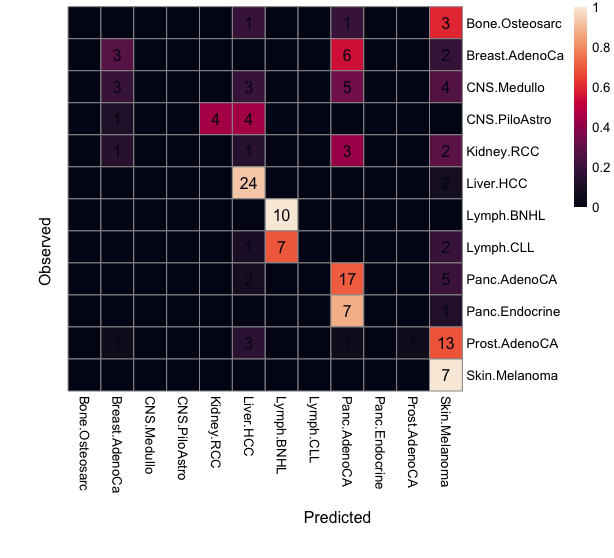
\includegraphics[width=\textwidth,height=0.9\textwidth]{graphics/confusion_matrix_bins_euclidean.png}
    \caption{Bin/Euclidean}
    \label{fig:confusion_bin_euclidean}
    \end{subfigure}
    ~
    \begin{subfigure}{.5\textwidth}
    \centering
    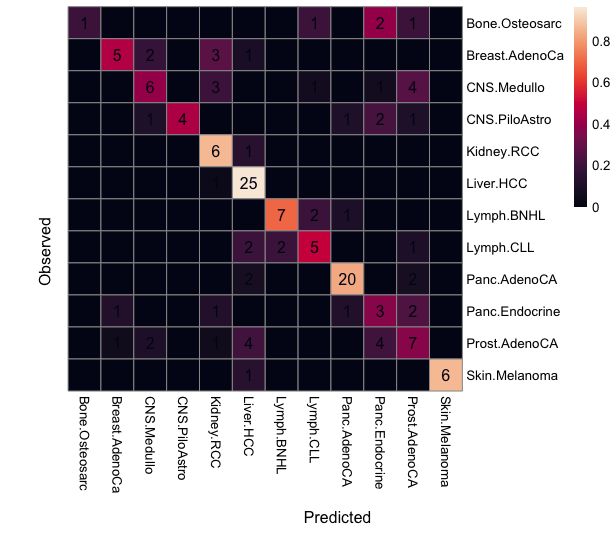
\includegraphics[width=\textwidth,height=0.9\textwidth]{graphics/confusion_matrix_smooth_euclidean.png}
    \caption{Smoothing/Euclidean}
    \label{fig:confusion_smooth_euclidean}
    \end{subfigure} \\
    \vspace{0.5cm}
    
    \begin{subfigure}{0.5\textwidth}
    \centering
    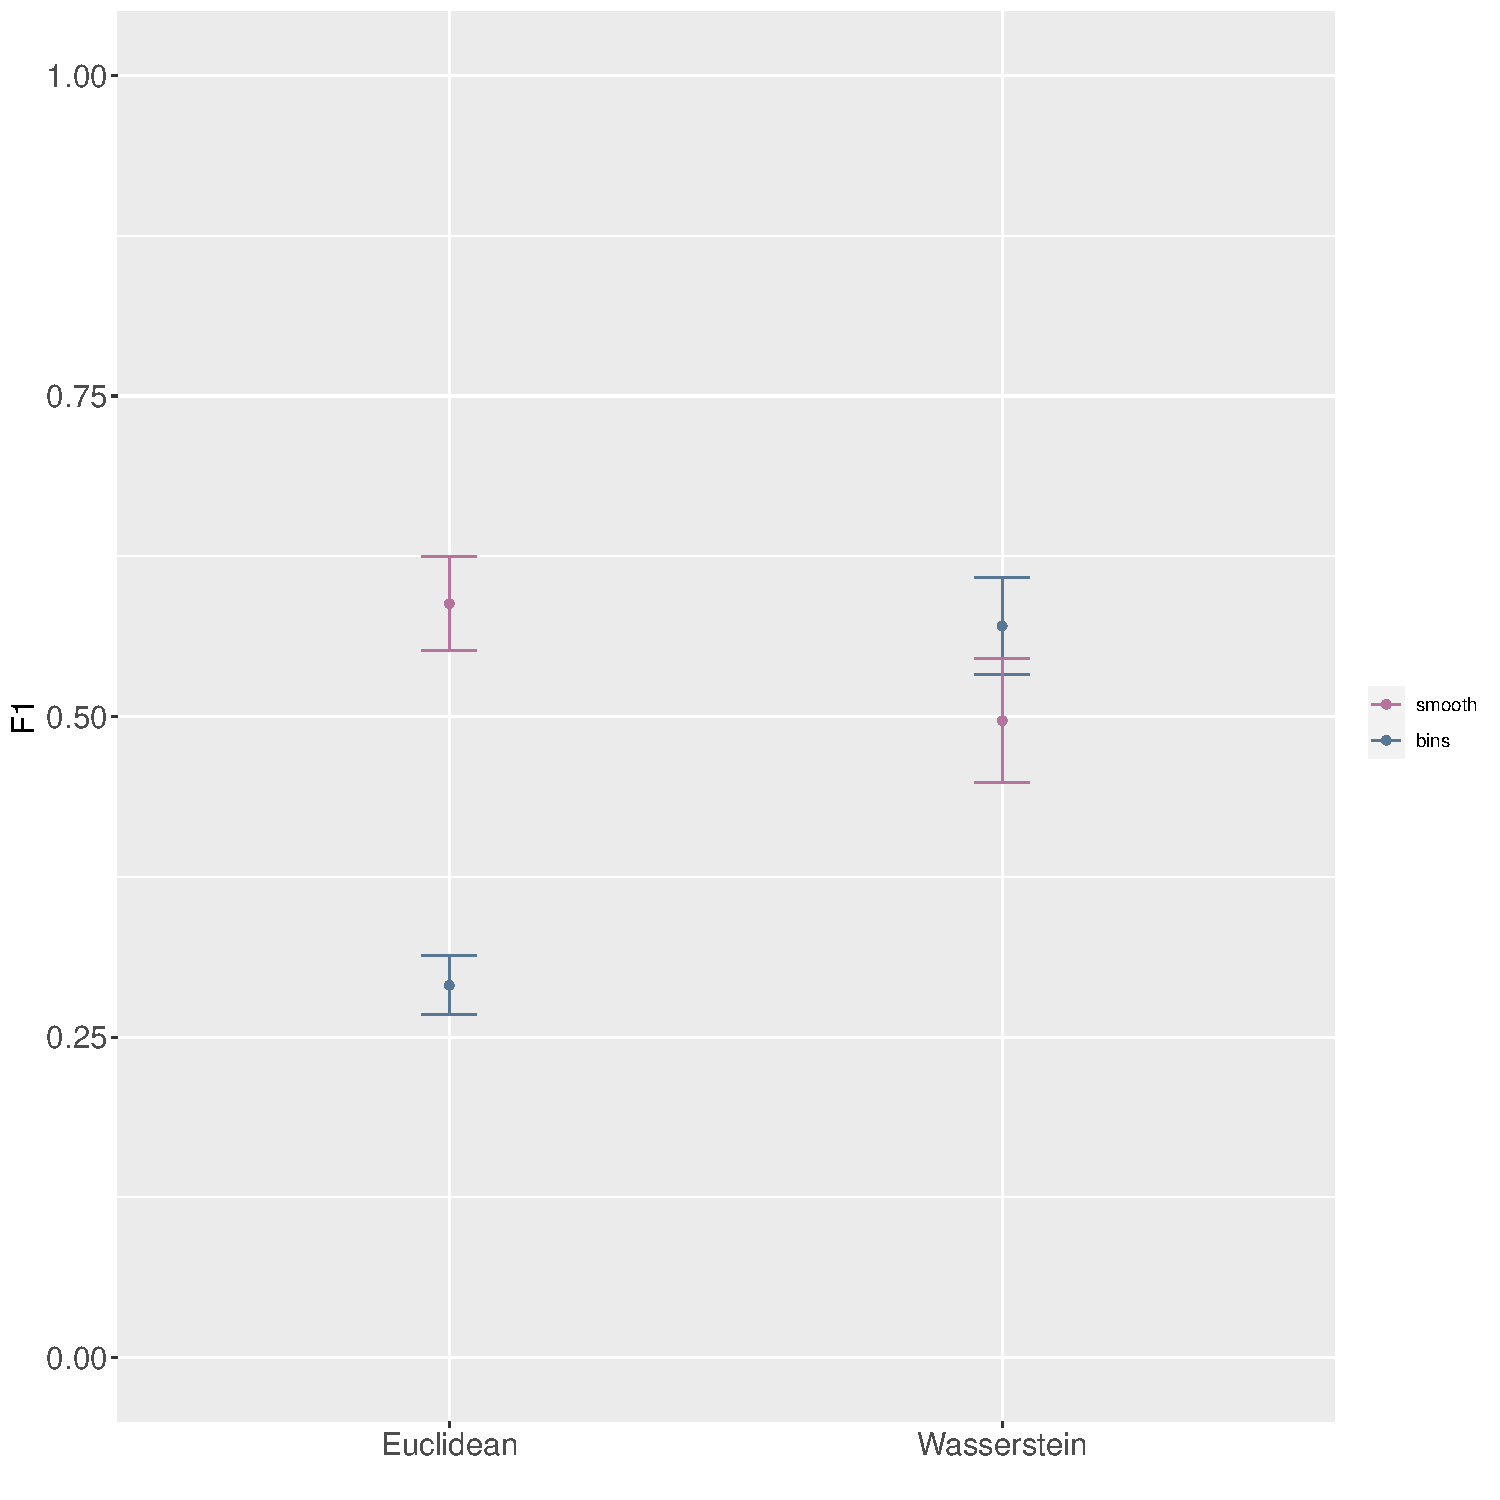
\includegraphics[scale=0.8]{graphics/f1_gle.pdf}
    \caption{F1 summary}
    \label{fig:f1_gle}
    \end{subfigure}
    
    
    \caption{\textbf{Smoothing was more accurate than binning for Euclidean distance, the difference between two representations was unclear for Wasserstein}. For each combination of representation/metric, I iterated the training procedures 10 times. Here, a representative confusion matrix, coloured by the percentage of predicted values over row total, is shown for (a) Bin/Euclidean, (b) Smooth/Euclidean. (c) shows the means of $F1$ for all representations/measures, the error bars are the standard errors for the iterated $F1$'s.}
    \label{fig:ml_gle}
\end{figure}

\section{Classifier based on SCE}\label{ml:sce}

\subsection{3-mer is the most accurate sequence context size}

\subsection{Dissecting 5-mer into submotifs can potentially improve accuracy}

\section{Classifier based on the combination of GLE and SCE}\label{ml:both}